\begin{figure}
\centering	
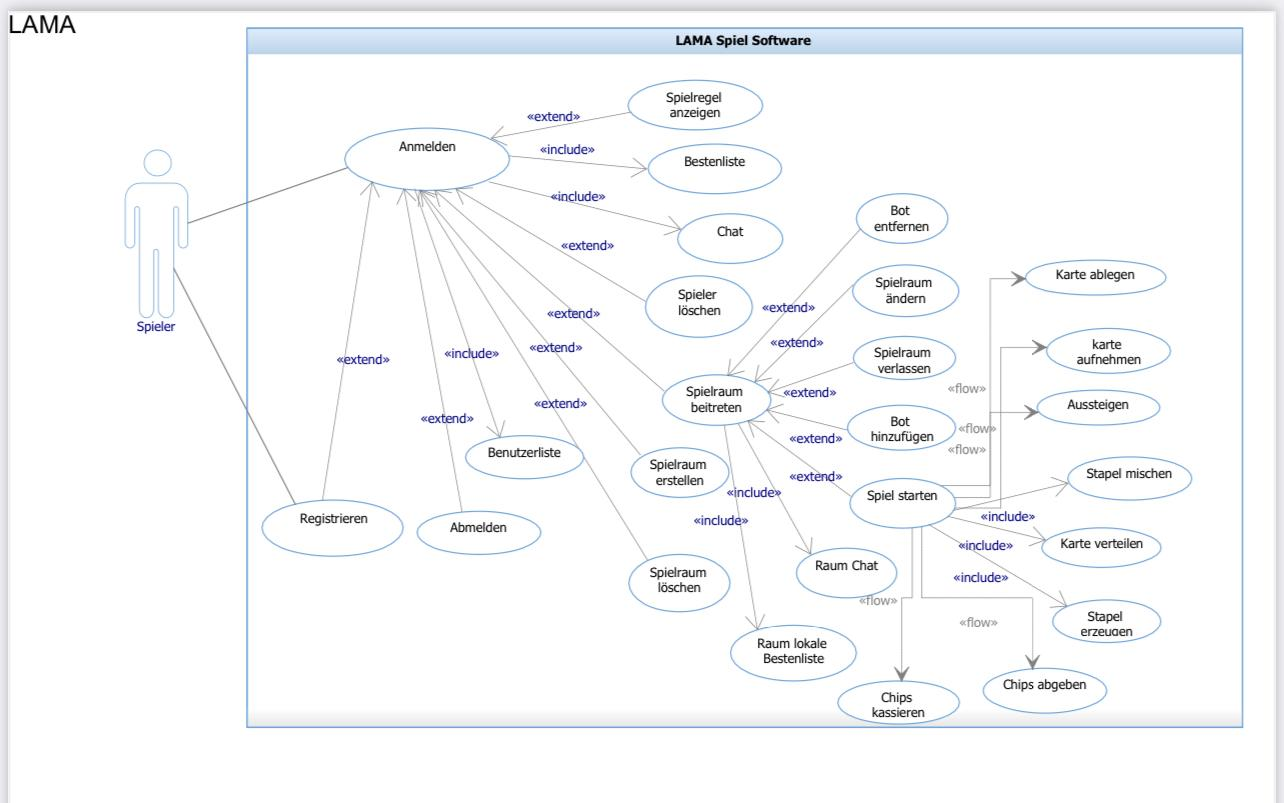
\includegraphics[width=0.9\textwidth]{img/UseCase1.jpeg}
\label{fig:sys}
\caption{Systemgrenzendiagramm (Use Case Diagramm)}
\end{figure}

\section{Systemgrenze (Use Case Diagramm)}

Die Systemgrenze wird in der Abbildung~\ref{fig:sys} dargestellt\footnote{Weitere Erklärungen und Spezifizierungen, die sich auf Abgrenzungen der Verantwortlichkeiten vom System und weiteren Akteuren/Systemen beziehen, können hier spezifiziert werden.}. 


\section{Beschreibungen der Anwendungsfälle}

\newcounter{uc}\setcounter{uc}{10}

\begin{description}[leftmargin=5em, style=sameline]

	\begin{lhp}{uc}{UC}{uc:registrieren} %name angepasst
		\item [Name:] Spieler registrieren
		\item [Ziel:] Spieler registrieren sich im System
		\item [Akteure:] Spieler.
		\item [Vorbedingungen:] Spieler ist in Vorraum und hat den Knopf "Registrieren" gedrückt um das Registrierungsinterface zu öffnen
		\item [Eingabedaten:] Zugriffsdaten \ref{daten:benutzername}~\ref{daten:passwort}.
		\item [Beschreibung:] Der Spieler füllt das Registrierungsformular aus und bestätigt die Eingaben mit dem Account erstellen Button, oder bricht die Registrierung mit dem Abbrechen Knopf ab.
		\item [Ausnahmen:] \hfill
			\begin{itemize} 
				\item[] \textit{Benutzername bereits vergeben:} Das System zeigt eine Fehlermeldung an.
				\item[] \textit{Passwort im $"$Feld Passwort$"$ und $"$Passwort Wdh$"$ stimmen nicht überein:} Das System zeigt eine Fehlermeldung an.
				\item[] \textit{Eines oder mehrere der Felder im Formular sind noch leer:} Das System zeigt eine Fehlermeldung an.
			\end{itemize}
		\item [Ergebnisse und Outputdaten:] Der Spieler ist registriert, befindet sich nun in der Lobby und sieht die Bestenliste.
		\item [Systemfunktionen] \ref{funk:zugriff}
	\end{lhp}

	
	\begin{lhp}{uc}{UC}{uc:anmelden} 
		\item [Name:] Spieler anmelden.
		\item [Ziel:] Spieler meldet sich im System an.
		\item [Akteure:] Spieler.
		\item [Vorbedingungen:] Spieler ist im Vorraum.
		\item [Eingabedaten:] Zugriffsdaten~\ref{daten:benutzername}~\ref{daten:passwort}.
		\item [Beschreibung:] Spieler meldet sich an.							
		\item [Ausnahmen:] \hfill
			\begin{itemize} 
				\item[] \textit{Passwort oder Benutzername ist falsch:} Das System zeigt eine Fehlermeldung an.
				\item[] \textit{Eines oder mehrere der Felder im Formular sind noch leer:} Das System zeigt eine Fehlermeldung an.
			\end{itemize}
		\item [Ergebnisse und Outputdaten:] Spieler ist in der Lobby und sieht die Bestenliste.	
		\item [Systemfunktionen:] \ref{funk:zugriff}.
	\end{lhp}
	
	\begin{lhp}{uc}{UC}{uc:abmelden} 
		\item [Name:] Spieler abmelden.
		\item [Ziel:] Spieler meldet sich im System ab.
		\item [Akteure:] Spieler.
		\item [Vorbedingungen:] Spieler ist in der Lobby
		\item [Eingabedaten:] -.
		\item [Beschreibung:] Spieler meldet sich ab.	
		\item [Ausnahmen:] -.
		\item [Ergebnisse und Outputdaten:]	Spieler wird in das Anmelden Interface bewegt.
		\item [Systemfunktionen:] \ref{funk:zugriff}.
	\end{lhp}
	
	\begin{lhp}{uc}{UC}{uc:löschen} %name angepasst
		\item [Name:] Spieler löschen.
		\item [Ziel:] Spieler entfernt seine Daten aus dem System.
		\item [Akteure:] Spieler
		\item [Vorbedingungen:] Spieler ist in der Lobby
		\item [Eingabedaten:] Passwort~\ref{daten:passwort}.
		\item [Beschreibung:]  Der Spieler füllt das Löschungssformular aus und bestätigt dies mit dem Bestätigen Button oder bricht den Vorgang ab
		\item [Ausnahmen:] \hfill
			\begin{itemize} 
				\item[] \textit{Passwort ist falsch}: Das system zeigt eine Fehlermeldung.
				\item[] \textit{Benutzername ist falsch}: Das System zeigt eine Fehlermeldung.
				\item[] \textit{Eines oder mehrere der Felder im Formular sind noch leer:} Das System zeigt eine Fehlermeldung an.
			\end{itemize}
		\item [Ergebnisse und Outputdaten:] Spieler ist im Vorraum, Spielerkonto wurde gelöscht.	
		\item [Systemfunktionen:] \ref{funk:zugriff}.
	\end{lhp}
	
	\begin{lhp}{uc}{UC}{uc:ablegen} %name angepasst
		\item [Name:] Karte ablegen.
		\item [Ziel:] Eine Karte wird abgelegt.
		\item [Akteure:] Spieler.
		\item [Vorbedingungen:] Spieler ist im Spielaum und an der Reihe.
		\item [Eingabedaten:] -. 
		\item [Beschreibung:] Spieler legt eine seiner Karten ab. Was der Spieler ablegen darf hängt von der obersten Karte des Ablagestapels ab. Die abgelegt Karte darf dabei nur eine Karte sein, deren Wert gleich, oder um eins höher ist als der Wert der Karte auf dem Ablagestapel. Ein Lama darf auf eine 6 oder ein anderes Lama gelegt werden, auf ein Lama darf ein weiteres Lama oder eine 1 gelegt werden.
		\item [Ausnahmen:] \hfill
		\begin{itemize} 
				\item[] \textit{Ausgewählte Karte ist nach Regelwerk ungültig}: Das system zeigt eine Fehlermeldung.
		\end{itemize}
		\item [Ergebnisse und Outputdaten:] Eine Karte wird auf dem Ablegestapel hinzugefügt und der Zug wird beendet.	
		\item [Systemfunktionen:] \ref{funk:spielverw}. %funk geändert
	\end{lhp}
	
	\begin{lhp}{uc}{UC}{uc:aufnehmen} %name angepasst
		\item [Name:] Karte aufnehmen.
		\item [Ziel:] Eine Karte wird aufgenommen.
		\item [Akteure:] Spieler.
		\item [Vorbedingungen:] Spieler ist im Spielraum, ist an der Reihe zu spielen, der Nachziehstapel ist nicht leer und es sind nicht bereits alle anderen Spieler aus dem Durchgang ausgestiegen.
		\item [Eingabedaten:] -. 
		\item [Beschreibung:] Spieler nimmt eine Karte auf, diese wird auf die Spielerhand hinzugefügt und aus dem Nachziehstapel gelöscht.
		\item [Ausnahmen:] -.
		\item [Ergebnisse und Outputdaten:] Eine Karte wird auf die Spielerhand hinzugefügt, aus dem Nachziehstapel entfernt und der Zug wird beendet.	
		\item [Systemfunktionen:] \ref{funk:spielverw}. %funk geändert
	\end{lhp}
    
	\begin{lhp}{uc}{UC}{uc:aussteigen} %name angepasst
		\item [Name:] Aussteigen.
		\item [Ziel:] Spieler steigt aus dem Durchgang aus.
		\item [Akteure:] Spieler.
		\item [Vorbedingungen:] Spieler ist im Spielraum und an der Reihe.
		\item [Eingabedaten:] -. 
		\item [Beschreibung:] Spieler legt seine Karten ab.
		\item [Ausnahmen:] -.
		\item [Ergebnisse und Outputdaten:] Spieler legt seine Karten verdeckt vor sich und der Durchgang ist für den Spieler beendet.	
		\item [Systemfunktionen:] \ref{funk:spielverw}. %funk geändert
	\end{lhp}
	
	\begin{lhp}{uc}{UC}{uc:srbeitreten} %name angepasst
		\item [Name:] Spielraum beitreten.
		\item [Ziel:] Spieler betritt den Spielraum.
		\item [Akteure:] Spieler.
		\item [Vorbedingungen:] Spieler ist in der Lobby.
		\item [Eingabedaten:] -.
		\item [Beschreibung:] Spieler betritt einen Spielraum. Die Spieler belegen die Plätze im Raum in folgender Reihenfolge: 1. Unten 2. Oben 3. Links-oben 4. Rechts-oben 5. Links-unten 6. Rechts-unten
		\item [Ausnahmen:] \hfill
		\begin{itemize} 
				\item[] \textit{Raum ist bereits voll:} Das System zeigt eine Fehlermeldung an.
				\item[] \textit{Raum ist nicht mehr vorhanden:} Das System zeigt eine Fehlermeldung an.
				\item[] \textit{Spiel bereits gestartet:} Das System zeigt eine Fehlermeldung an.
			\end{itemize}
		\item [Ergebnisse und Outputdaten:] Spieler betritt den Spielraum.	
		\item [Systemfunktionen:] \ref{funk:spielraum}. %funk geändert
	\end{lhp}
	
	\begin{lhp}{uc}{UC}{uc:srverlassen} %name angepasst
		\item [Name:] Spielraum verlassen.
		\item [Ziel:] Spieler verlässt den Spielraum.
		\item [Akteure:] Spieler.
		\item [Vorbedingungen:] Spieler ist im Spielraum und das Spiel hat noch nicht begonnen.
		\item [Eingabedaten:] -.
		\item [Beschreibung:] Spieler verlässt einen Spielraum.
		\item [Ausnahmen:]
        -.
		\item [Ergebnisse und Outputdaten:] Spieler verlässt den Spielraum.	Die aktuelle Spieleranzahl im verlassenen Raum wird um eins verringert und der Slot des Spielers wird wieder freigegeben. Spieler, die dem Raum erst nach dem Spieler, der den Raum verlassen hat, beigetreten sind werden um jeweils einen Platz nach vorne verschoben (siehe \ref{uc:srbeitreten}). Ist der Spieler der Host des Spielraums, so verlassen alle Spieler automatisch den Raum.
		\item [Systemfunktionen:] \ref{funk:spielraum}. %funk geändert
	\end{lhp}
	
	
	\begin{lhp}{uc}{UC}{uc:srerstellen} %name angepasst
		\item [Name:] Spielraum erstellen.
		\item [Ziel:] Spielraum wird erstellt.
		\item [Akteure:] Spieler.
		\item [Vorbedingungen:] Spieler ist in der Lobby.
		\item [Eingabedaten:] Raumname \begin{comment}
		\ref{daten:raumname}
		\end{comment}
		\item [Beschreibung:] Der Spieler füllt das Formular zum erstellen eines Spielraums aus und bestätigt dies mit dem Bestätigen Button oder bricht den Vorgang ab
		\item [Ausnahmen:] \hfill
		\begin{itemize} 
				\item[] \textit{Raumname ist vergeben:} Das System zeigt eine Fehlermeldung an.
				\item[] \textit{Die Spieleranzahl liegt nicht zwischen 2 und 6:} Das System zeigt eine Fehlermeldung an.
				\item[] \textit{Eines oder mehrere der Felder im Formular sind noch leer:} Das System zeigt eine Fehlermeldung an.
			\end{itemize}
		\item [Ergebnisse und Outputdaten:] Der Raum wurde erstellt.	
		\item [Systemfunktionen:] \ref{funk:spielraum}. %funk geändert
	\end{lhp}
	
	 \begin{lhp}{uc}{UC}{uc:starten} %name angepasst
		\item [Name:] Spiel starten.
		\item [Ziel:] LAMA Spielrunde starten.
		\item [Akteure:] Spieler.
		\item [Vorbedingungen:] Spieler ist im Spielraum und ist der Host dieses, befindet sich in diesem und der Raum ist voll.
		\item [Eingabedaten:] -.
		\item [Beschreibung:] Eine LAMA Spielrunde wird gestartet.
		\item [Ausnahmen:] -.
		\item [Ergebnisse und Outputdaten:] Spielrunde wird gestartet, Karten werden gemischt und den Spielern verteilt, oberste Karte des Nachziehstapels wird im Ablagestapel hinzugefügt und ein zufälliger Spieler beginnt mit seinem ersten Zug.
		\item [Systemfunktionen:] \ref{funk:spielverw}. %funk geändert
	\end{lhp}
	
	 
	\begin{lhp}{uc}{UC}{uc:srändern} %name angepasst
		\item [Name:] Spielraum ändern.
		\item [Ziel:] Spielraum wird geändert.
		\item [Akteure:] Spieler.
		\item [Vorbedingungen:] Spieler ist Host des Spielraums und befindet sich in diesem
		\item [Eingabedaten:] -.
		\item [Beschreibung:] Host ändert die Einstellungen (Raumname, Raumgröße) des Spielraums, oder bricht den Vorgang ab.
		\item [Ausnahmen:] \hfill
		\begin{itemize} 
				\item[] \textit{Es sind aktuell mehr Spieler im Spiel, als die neu eingestellte maximale Spieleranzahl erlaubt, oder die Spieleranzahl liegt nicht zwischen 2 und 6 :} Das System zeigt eine Fehlermeldung an.
				\item[] \textit{Raumname ist vergeben:} Das System zeigt eine Fehlermeldung an.
				\item[] \textit{Eines oder mehrere der Felder im Formular sind noch leer:} Das System zeigt eine Fehlermeldung an.
	  \end{itemize}
		\item [Ergebnisse und Outputdaten:] Der Raum wurde geändert.	
		\item [Systemfunktionen:] \ref{funk:spielraum}. 
	\end{lhp}
	
	\begin{lhp}{uc}{UC}{uc:srlöschen} 
		\item [Name:] Spielraum löschen.
		\item [Ziel:] Spielraum wird gelöscht.
		\item [Akteure:] Spieler. 
		\item [Vorbedingungen:] Spieler ist Host des Spielraumes, befindet sich in diesem und das Spiel wurde noch nicht gestartet. 
		\item [Eingabedaten:]  -.
		\item [Beschreibung:] Host löscht den Spielraum, in welchem er sich befindet , oder bricht den Vorgang ab.
		\item [Ausnahmen:] -. 
		\item [Ergebnisse und Outputdaten:] Der Raum wird gelöscht und alle noch im Raum verbleibenden Spieler werden in die Lobby verschoben.	
		\item [Systemfunktionen:] \ref{funk:spielraum}. 
	\end{lhp}
	
	\begin{lhp}{uc}{UC}{uc:bestenliste} %name angepasst
		\item [Name:] Bestenliste anzeigen.
		\item [Ziel:] Die Anzahl der gewonnen Spiele aller Spieler raumübergreifend anzeigen.
		\item [Akteure:] -.
		\item [Vorbedingungen:] Spieler ist angemeldet und befindet sich in der Lobby.
		\item [Eingabedaten:] -.
		\item [Beschreibung:] Spieler befindet sich in der Lobby und kann die Bestenliste sehen.
		\item [Ausnahmen:] -.
		\item [Ergebnisse und Outputdaten:] Liste der aktuellen besten Spielern wird angezeigt.
		\item [Systemfunktionen:] \ref{funk:bestenliste}. %funk geändert
	\end{lhp}
	
		\begin{lhp}{uc}{UC}{uc:raumbestenliste} %name angepasst
		\item [Name:] Raum-lokale Bestenliste anzeigen.
		\item [Ziel:] Die Anzahl der gewonnen Spiele aller Spieler im Spielraum anzeigen.
		\item [Akteure:] Spieler.
		\item [Vorbedingungen:] Spieler befindet sich im Spielraum.
		\item [Eingabedaten:] -.
		\item [Beschreibung:]  Es wird die Bestenliste des Spielraums angezeigt.
		\item [Ausnahmen:] -.
		\item [Ergebnisse und Outputdaten:]  Das Bestenliste-Interface öffnet sich.
		\item [Systemfunktionen:] \ref{funk:bestenliste}. %funk geändert
	\end{lhp}
	
	\begin{lhp}{uc}{UC}{uc:bots}
		\item [Name:] Bot hinzufügen.
		\item [Ziel:] Intelligente Bots im Spiel hinzufügen.
		\item [Akteure:] Spieler. 
		\item [Vorbedingungen:]  Spieler ist Host eines Spielraums und befindet sich in diesem. Der Raum ist noch nicht voll.
		\item [Eingabedaten:] -. %siehe /LF50/
		\item [Beschreibung:] Host wählt den Schwierigkeitsgrad der Bots aus und fügt diese dem Spiel hinzu.
		\item [Ausnahmen:] -.
		\item [Ergebnisse und Outputdaten:] Bots werden dem Spielraum hinzugefügt.
		\item [Systemfunktionen:] \ref{funk:bots}. %funk geändert
	\end{lhp}
	
	\begin{lhp}{uc}{UC}{uc:botsentfernen}
		\item [Name:] Bot entfernen.
		\item [Ziel:] Intelligente Bots aus dem Spiel entfernen.
		\item [Akteure:] Spieler. 
		\item [Vorbedingungen:]  Spieler ist Host eines Spielraums und befindet sich in diesem. Das Spiel ist noch nicht gestartet und es befinden sich  bereits Bots des zu entfernenden Typs im Spielraum.
		\item [Eingabedaten:] -. %siehe /LF50/
		\item [Beschreibung:] Host wählt den Schwierigkeitsgrad des zu entfernen Bots aus und entfernt diese dem Spiel.
		\item [Ausnahmen:] -.
		\item [Ergebnisse und Outputdaten:] Bots werden aus dem Spielraum entfernt, Anzahl der Spieler wird um eins geringer und ein Slot wird freigegeben.
		\item [Systemfunktionen:] \ref{funk:bots}. %funk geändert
	\end{lhp}
	
	\begin{lhp}{uc}{UC}{uc:chat} %name angepasst
		\item [Name:] Chat.
		\item [Ziel:] Chatfenster wird erzeugt.
		\item [Akteure:] Spieler.
		\item [Vorbedingungen:] Spieler in der Lobby.
		\item [Eingabedaten:] -. %Spieler interagiert mit den "Etwas schreiben" Teil?
		\item [Beschreibung:] Spieler in der Lobby können mit einander kommunizieren.
		\item [Ausnahmen:] -.
		\item [Ergebnisse und Outputdaten:] Nachrichten werden an andere Spieler in der Lobby geschickt, Nachrichten anderer Spieler in der Lobby, so wie die eigenen werden angezeigt.	
		\item [Systemfunktionen:] \ref{funk:chat}. %funk geändert
	\end{lhp}
	
		\begin{lhp}{uc}{UC}{uc:srchat} %name angepasst
		\item [Name:] Raum Chat.
		\item [Ziel:] Chatfenster im Spielraum wird erzeugt.
		\item [Akteure:] Spieler.
		\item [Vorbedingungen:] Spieler ist im Spielraum.
		\item [Eingabedaten:] -. %Spieler interagiert mit den "Etwas schreiben" Teil?
		\item [Beschreibung:] Spieler können mit einander kommunizieren.
		\item [Ausnahmen:] -.
			
		\item [Ergebnisse und Outputdaten:] Nachrichten werden an andere Spieler im Spielraum geschickt, Nachrichten anderer Spieler im Spielraum, so wie die eigenen werden angezeigt.	
		\item [Systemfunktionen:] \ref{funk:chat}. %funk geändert
	\end{lhp}


	\begin{lhp}{uc}{UC}{uc:chipskassieren} 
		\item [Name:] Chips kassieren.
		\item [Ziel:] Spieler kassiert Minuspunkte in Form von Chips für verbliebene Karten.
		\item [Akteure:] -.
		\item [Vorbedingungen:]Spieler befindet sich im Spiel, hat noch verbleibende Karten und der aktuelle Durchgang ist beendet.Das Spiel ist im Gange und der aktuelle Durchgang ist beendet.
		\item [Eingabedaten:] -. 
		\item [Beschreibung:] Der Spieler kassiert Chips für in der Hand oder auf dem Tisch verbliebene Karten. Die Minuspunkte für eine Karte entsprechen dem Kartenwert dieser. Lamas zählen 10 Minuspunkte. Jeder Kartenwert zählt nur einmal.Die Spieler kassieren Chips für ihre in der Hand oder auf dem Tisch verbliebene Karten. Die Minuspunkte für eine Karte entsprechen dem Kartenwert dieser. Lamas zählen 10 Minuspunkte. Jeder Kartenwert zählt nur einmal
		\item [Ausnahmen:] -.
		\item [Ergebnisse und Outputdaten:] Jeder Spieler kassiert 1er und/oder 10er Chips entsprechend seiner Minuspunkte. Anzahl der Chips des Spielers erhöht sich dem entsprechend. Es werden zuerst 10er Chips vergeben, der Rest der Minuspunkte wird dann mit 1er Chips ausgegeben.
		\item [Systemfunktionen:] \ref{funk:spielverw}.
	\end{lhp}
	
	\begin{lhp}{uc}{UC}{uc:chipsabgeben} 
		\item [Name:] Chips abgeben.
		\item [Ziel:] Spieler gibt Minuspunkte in Form von Chips ab
		\item [Akteure:] Spieler.
		\item [Vorbedingungen:] Spieler befindet sich im Spiel, hat alle seine Karten auf den Ablagestapel gelegt und besitzt mindestens einen der zur Auswahl stehenden Chips.
		\item [Eingabedaten:] -. 
		\item [Beschreibung:] Der Spieler gibt einen Chip ab, es kann ein 1er oder ein 10er Chip sein, insofern er diesen besitzt.
		\item [Ausnahmen:] -.
		\item [Ergebnisse und Outputdaten:] Spieler gibt einen 1er oder 10er Chip ab. Die Anzahl des gewählten Typs an Chips des Spielers (1er oder 10er Chips) wird um eins reduziert.
		\item [Systemfunktionen:] \ref{funk:spielverw}.
	\end{lhp}
	
		\begin{lhp}{uc}{UC}{uc:benutzerliste} 
		\item [Name:] Benutzerliste anzeigen.
		\item [Ziel:] Zeigt die Liste der aktuell angemeldeten Benutzer an.
		\item [Akteure:] Spieler.
		\item [Vorbedingungen:] Spieler befindet sich in der Lobby und klickt auf das entsprechende Icon.
		\item [Eingabedaten:] -. 
		\item [Beschreibung:] Zeigt die Liste der aktuell angemeldeten Benutzer an.
		\item [Ausnahmen:] -.
		\item [Ergebnisse und Outputdaten:] Zeigt die Liste der aktuell angemeldeten Benutzer an.	
		\item [Systemfunktionen:] \ref{funk:spielverw}.
	\end{lhp}

	\begin{lhp}{uc}{UC}{uc:deck} %name angepasst
		\item [Name:] Stapel erstellen.
		\item [Ziel:] Stapel mit LAMA Spielkarten erzeugen.
		\item [Akteure:] -.
		\item [Vorbedingungen:] Spiel wird gestartet. 
		\item [Eingabedaten:] -.
		\item [Beschreibung:] Es wird ein Stapel mit Spielkarten erzeugt.
		\item [Ausnahmen:] -.
		\item [Ergebnisse und Outputdaten:] Stapel wird erzeugt, dieser besteht aus 8 mal Karten der Werten 1-6 und 8 Lama-Karten.
		\item [Systemfunktionen:] \ref{funk:spielverw}. %funk geändert
	\end{lhp}

	\begin{lhp}{uc}{UC}{uc:mischen} %name angepasst
		\item [Name:] Stapel mischen.
		\item [Ziel:] Neu erzeugter Stapel wird gemischt.
		\item [Akteure:] -.
		\item [Vorbedingungen:] Spiel ist gestartet, Kartenstapel ist erzeugt. 
		\item [Eingabedaten:]  -.
		\item [Beschreibung:] Stapel wird gemischt.
		\item [Ausnahmen:] -.
		\item [Ergebnisse und Outputdaten:] Neu erzeugter Stapel mit LAMA Spielkarten wird gemischt, die Position der Karten im Stapel ist also randomisiert.	
		\item [Systemfunktionen:] \ref{funk:spielverw}. %funk geändert
	\end{lhp}
	
	\begin{lhp}{uc}{UC}{uc:verteilen} %name angepasst
		\item [Name:] Karten verteilen.
		\item [Ziel:] Jeder Spieler bekommt 6 Spielkarten.
		\item [Akteure:] -.
		\item [Vorbedingungen:] Spiel ist gestartet, Kartenstapel ist erzeugt und gemischt. 
		\item [Eingabedaten:] -.
		\item [Beschreibung:] 6 Spielkarten werden auf dem Hand jedes Spielers hinzugefügt und die werden aus dem Stapel (Nachziehstapel) gelöscht. Eine weitere Karte wird auf dem Ablegestapel hinzugefügt.
		\item [Ausnahmen:] -.
		\item [Ergebnisse und Outputdaten:] Neu erzeugter Stapel mit LAMA Spielkarten wird gemischt.	
		\item [Systemfunktionen:] \ref{funk:spielverw}. %funk geändert
	\end{lhp}
	
    \begin{lhp}{uc}{UC}{uc:regeln} %name angepasst
		\item [Name:] Spielregeln anzeigen. 
		\item [Ziel:] Zeigt die Spielregeln von LAMA an.
		\item [Akteure:] Spieler 
		\item [Vorbedingungen:] Spieler befindet sich in der Lobby.
		\item [Eingabedaten:] -.
		\item [Beschreibung:] Das Regelwerk von LAMA wird angezeigt.
		\item [Ausnahmen:] -.
		\item [Ergebnisse und Outputdaten:] Es öffnet sich das Spielregeln Interface.
		\item [Systemfunktionen:] \ref{funk:regel}. 
	\end{lhp}	

	
	
	
	
	
	

\end{description}